\documentclass[11pt]{article}

% ----------------------------------------------------------------- packages
\usepackage[margin=1in]{geometry}
\usepackage{amsmath,amssymb,amsthm}
\usepackage{graphicx}
\usepackage{booktabs}
\usepackage{xcolor}
\usepackage{caption}
\usepackage{subcaption}
\usepackage{enumitem}
\usepackage{algorithm}
\usepackage{algpseudocode}
\usepackage{microtype}
\usepackage[colorlinks=true,linkcolor=blue!55!black,citecolor=blue!55!black,urlcolor=blue!55!black]{hyperref}

\captionsetup{font=small,labelfont=bf}
\captionsetup[sub]{font=small}
\graphicspath{{figures/}}

\definecolor{sig}{HTML}{1a7a3a}
\newcommand{\sigmark}[1]{\textcolor{sig}{\textbf{#1}}}
\newcommand{\Ecal}{\mathcal{E}}
\newcommand{\Hcal}{H}
\newcommand{\Var}{\operatorname{Var}}
\newcommand{\Cov}{\operatorname{Cov}}
\newcommand{\R}{\mathbb{R}}
\newcommand{\E}{\mathbb{E}}
\newcommand{\code}[1]{\texttt{\small #1}}

\newtheorem{proposition}{Proposition}

\title{\textbf{Score-Identified Distributional Dynamics on \textit{C.\ elegans}}\\[2pt]
\large A conditional-law functional connectome and a significant, biologically-coherent
lag-resolved signature the conditional mean cannot express}
\author{}
\date{\today}

\begin{document}
\maketitle
\vspace{-2.5em}

\begin{abstract}
\noindent
Standard functional-connectivity and causal-discovery methods estimate a \emph{conditional mean}:
how one neuron's activity predicts another's future level. They are, by construction, blind to
\emph{distributional} interactions --- how one neuron modulates the \emph{variance}, gain, or tails
of another's predictive law --- which is exactly the regime in which slow, metabotropic and
peptidergic neuromodulation is expected to act. We develop \textbf{score-identified dynamics}
(SID): we estimate the full one-step conditional predictive density $\rho(y\mid \Hcal_t)$ with a
convex, closed-form quadratic-score estimator, and read out directed \emph{mean}, \emph{gain}
($\partial\log\Var$), and \emph{tail} channels as derivative-free covariances against the
conditional score. On a synthetic hidden-thermostat system the gain channel recovers a
conditional-variance memory kernel that is provably invisible to every conditional-mean method
(kernel correlation $0.998$ vs.\ the Kalman oracle; mean-model $R^2\approx0$). We then apply SID to
whole-brain NeuroPAL calcium imaging, after auditing the prior SBTG pipeline (29 confirmed bugs)
and fixing a connectome-orientation bug that had invalidated its reported numbers. Evaluated
\emph{holistically} across an ensemble of noisy anatomical and receptor-expression targets, SID's
mean channel is the equal-best single method (mean rank tied with pairwise correlation), and its
non-Gaussian variant delivers the single strongest result exactly where theory predicts
(metabotropic serotonin, AUROC $0.78$). The central real-data result is \emph{lag-resolved and
relative}: within the same fit, the distributional channels' correspondence to the slow peptidergic
neuromodulator network shifts toward \emph{longer lags} than the mean channel's ($\Delta$ log-slope
$+0.0079$, 95\% CI $[+0.0025,+0.0120]$ for gain at maximum reference power), while the same contrast
is null for the wired connectome --- a channel$\times$reference double dissociation no mean-only
method can produce. We then subject this single finding to a deliberate battery (\S\ref{sec:robust}):
it is specific to \emph{partial} conditioning (it reverses marginally); its statistical significance
is \emph{power-limited} (clear only in the 80-neuron / 757-edge configuration --- directionally
consistent but not individually significant as neurons are traded for worms across 6--28 animals and
two imputation schemes); and, decisively, it is \textbf{not an estimator artifact} --- a
circular-shift surrogate that destroys cross-neuron coupling collapses the contrast to zero, with the
observed value in the tail ($p=0.008$). It is, however, \emph{single-instrument}: a cruder non-SID
variance estimator does not corroborate it. We therefore report it at exactly that altitude --- a
real, partial, surrogate-validated but as-yet single-instrument signal --- rather than over-claiming.
Along the way we retract an early ``tyramine'' over-claim that a trivial source-variance baseline
fully explained, and document the controls-first methodology that caught it (and that the surrogate
null extends).
\end{abstract}

% =====================================================================
\section{Problem statement}
\label{sec:problem}

The \textit{C.\ elegans} nervous system runs two signalling systems on top of the same 302 neurons:
a fast, wired system of chemical synapses and gap junctions (the ``connectome''), and a slow,
largely \emph{extrasynaptic} system of monoamines and neuropeptides that diffuse to distant
targets bearing cognate G-protein--coupled receptors (GPCRs). The wired system is well described by
how one neuron's activity \emph{drives the level} of another's --- a conditional-\emph{mean} effect.
The neuromodulatory system, by contrast, is expected to act on \emph{excitability and gain}: a
modulator does not so much set a target's next value as reshape the \emph{distribution} of what the
target can do next --- its variance, its propensity to burst, the heaviness of its tails.

Every workhorse method for inferring functional interactions from neural time series --- lagged
cross-correlation, multivariate/partial ridge regression, vector autoregression (VAR), VAR-LiNGAM,
SINDy, PCMCI$+$, DYNOTEARS, and the transfer-model $\hat\mu$ of the prior SBTG pipeline --- targets
the conditional mean $\E[y\mid \Hcal]$. \emph{None of them has a channel for a variance/gain/tail
effect.} If neuromodulation is primarily distributional, these methods are structurally the wrong
instrument, and a negative or mediocre result from them says little about whether the modulatory
structure is present in the data.

This work asks a sharpened question. Not ``does a new method beat the baselines at recovering a
single network'' --- the available biological targets are noisy proxies (anatomy is not function;
the ``monoamine/neuropeptide networks'' are receptor-expression \emph{predictions}, not measured
signalling), so a near-perfect AUROC on any one of them is an over-fit red flag, not a triumph.
Instead:
\begin{enumerate}[topsep=2pt,itemsep=1pt]
  \item Can we estimate the \emph{full conditional predictive law} of neural activity, and read out
        \emph{distributional} interaction channels that mean-based methods cannot represent?
  \item On synthetic systems with known ground truth, do those channels recover structure that is
        provably invisible to the mean?
  \item On real whole-brain data, evaluated fairly across the whole ensemble of imperfect targets,
        is the approach \emph{overall} competitive, and do the distributional channels add
        \emph{targeted} value exactly where slow modulation should live --- in a form robust to
        proxy noise?
\end{enumerate}
The standard of evidence is threefold: \textbf{principled}, \textbf{compelling on synthetics}, and
\textbf{overall competitive-to-better on real data in a relative, lag-resolved form}.

% =====================================================================
\section{Proposed approach and theory}
\label{sec:theory}

\subsection{Estimand: the conditional predictive law and its lag-influence score}
Let $x_t\in\R^N$ be the (pre-processed) activity of $N$ neurons and $\Hcal_t$ the history up to $t$.
The estimand is the one-step predictive density of a target coordinate,
\[
  \rho\bigl(y \mid \Hcal_t\bigr), \qquad y = x_{j}(t{+}\ell),
\]
\emph{not} merely its conditional mean $\mu_j(t)=\E[y\mid\Hcal_t]$. The central object is the
\textbf{lag-influence score}
\[
  \ell_u(y;h) \;=\; \nabla_{x_{t+1-u}}\log\rho(y\mid h),
\]
the sensitivity of the predictive log-density to the activity of a source $u$ steps back. Effects on
the mean, variance, tails, or any smooth statistic $T(y)$ are recovered as \textbf{covariances
against the score} (a Stein-type identity),
\[
  \frac{\partial\,\E[T(y)\mid h]}{\partial x_{t+1-u,i}}
  \;=\; \Cov\!\bigl(T(y),\,\ell_{u,i}(y;h)\bigr),
\]
so a distributional readout never requires differentiating a fitted black box --- it is a moment of
the score. This is what makes the framework both interpretable and cheap.

\subsection{A convex closed-form estimator}
We use a Gaussian conditional whose \emph{natural parameters are linear in features}
$\psi(t)\in\R^P$ (here $\psi=[1,\,x_0(t),\dots,x_{N-1}(t)]$, all sources' current activity):
\[
  y\mid\Hcal_t \sim \mathcal{N}\!\bigl(\mu(t), v(t)\bigr),\qquad
  \eta_1(t)=\theta_1^\top\psi(t),\quad \eta_2(t)=\theta_2^\top\psi(t),
\]
with sufficient statistic $T(y)=(y,y^2)$, conditional score $s_\theta(y,h)=\eta_1+2\eta_2 y$, and
\[
  v_{\mathrm{eff}}(t)=-\tfrac{1}{2\eta_2(t)},\qquad
  v(t)=v_{\mathrm{eff}}(t)-\sigma^2,\qquad
  \mu(t)=\eta_1(t)\,v_{\mathrm{eff}}(t).
\]
Because both Hyv\"arinen and denoising score matching are \emph{quadratic} in $\theta$, fitting is a
single regularized linear solve --- no optimizer, no local minima, no learning-rate confounds
(Algorithm~\ref{alg:qsm}). This is the disentangled conditional head of a two-head design realized
in closed form.

\begin{proposition}[Closed-form score matching]
For the quadratic-$T$ family above, the (denoising or Hyv\"arinen) score-matching objective is a
convex quadratic in $\theta=[\theta_1,\theta_2]$, with the unique minimizer given in
Algorithm~\ref{alg:qsm}.
\end{proposition}

\begin{algorithm}[t]
\caption{Closed-form quadratic-$T$ conditional score matcher (one target)}
\label{alg:qsm}
\begin{algorithmic}[1]
\Require targets $Y\in\R^{T}$, features $\Psi\in\R^{T\times P}$, ridge $\lambda\ge0$, noise $\sigma\ge0$
\If{$\sigma>0$} \Comment{denoising score matching}
  \State draw $\zeta\sim\mathcal{N}(0,I_T)$;\; $\tilde Y \gets Y+\sigma\zeta$;\; $g \gets \zeta/\sigma$
  \State $U \gets [\,\Psi,\; 2\,\tilde Y\odot\Psi\,]\in\R^{T\times 2P}$;\quad $A \gets U^\top U/T$;\quad $b \gets U^\top g/T$
  \State $\theta \gets -(A+\lambda I)^{-1} b$
\Else \Comment{Hyv\"arinen score matching, $\sigma=0$}
  \State $U \gets [\,\Psi,\; 2\,Y\odot\Psi\,]$;\quad $A \gets U^\top U/T$;\quad $c \gets [\,0_P,\; 2\,\overline{\Psi}\,]$
  \State $\theta \gets -(A+\lambda I)^{-1} c$ \Comment{$\overline\Psi=$ column means of $\Psi$}
\EndIf
\State \Return $\theta=[\theta_1,\theta_2]$ \Comment{per-sample estimating functions $\xi_t$ retained for HAC/sandwich inference}
\end{algorithmic}
\end{algorithm}

\subsection{Directed distributional readouts}
Fit one model per target $j$ at lag $\ell$ on features centered at the pooled history mean, so at the
``typical history'' the source features are $0$ and $\eta_1=\theta_1^{(0)}$, $\eta_2=\theta_2^{(0)}$
(intercept terms). Differentiating the closed-form moments with respect to source $i$ gives the
directed coupling matrices (all in the $[\text{post},\text{pre}]=[\text{target},\text{source}]$
convention), which are the entries of Algorithm~\ref{alg:readout}:
\[
\begin{aligned}
D_{\text{mean}}[j,i] &= v_{\mathrm{eff}}\,\theta_{1,i} + 2\,\eta_1 v_{\mathrm{eff}}^2\,\theta_{2,i}
   &&= \partial\,\E[y_j]/\partial x_i \quad\text{(VAR-comparable drive)}\\
D_{\text{gain}}[j,i] &= \bigl(2 v_{\mathrm{eff}}^2\,\theta_{2,i}\bigr)/v
   &&= \partial\log\Var[y_j]/\partial x_i \quad\text{(gain / excitability)}\\
D_{\text{tail}\uparrow}[j,i] &= \phi(a_{\uparrow})\!\left(\tfrac{D_{\text{mean}}}{\sqrt v}
   + \tfrac{q_{\uparrow}-\mu}{2 v^{3/2}} D_{\text{var}}\right)
   &&= \partial\,\Pr(y_j>q_{\uparrow})/\partial x_i \quad\text{(burst)}
\end{aligned}
\]
and symmetrically for the lower tail $D_{\text{tail}\downarrow}$, with
$a_{\uparrow}=(q_{\uparrow}-\mu)/\sqrt v$ and $D_{\text{var}}=2v_{\mathrm{eff}}^2\theta_{2}$. The
\emph{mean} channel is what a VAR/regression method also estimates; the \emph{gain} and \emph{tail}
channels have no classical analog.

\begin{algorithm}[t]
\caption{Distributional functional connectome at lag $\ell$}
\label{alg:readout}
\begin{algorithmic}[1]
\Require per-worm matrices $\{X^{(w)}\}$, neuron names, lag $\ell$, ridge $\lambda$
\For{each target $j=1,\dots,N$}
  \State pool $(Y,\Psi)$ across worms: $Y=x_j(t{+}\ell)$, $\Psi=[1,\,x(t)-\overline{x}]$ \Comment{no cross-worm windows}
  \State $\theta \gets$ Algorithm~\ref{alg:qsm}$(Y,\Psi,\lambda,\sigma{=}0)$;\quad set $q_\uparrow,q_\downarrow$ = 90/10\% quantiles of $Y$
  \State read $D_{\text{mean}}[j,\cdot],D_{\text{gain}}[j,\cdot],D_{\text{tail}\uparrow/\downarrow}[j,\cdot]$ at centered history; zero the diagonal
\EndFor
\State \Return channel matrices $\{D_{\text{mean}},D_{\text{gain}},D_{\text{tail}}\}$, each $[\text{post},\text{pre}]$
\end{algorithmic}
\end{algorithm}

% =====================================================================
\section{Synthetic validation: the gain channel sees what the mean cannot}
\label{sec:synth}

The decisive test uses a hidden-thermostat / stochastic-volatility process that is \emph{white with
zero conditional mean} --- so VAR, SINDy, and neural least-squares see nothing --- yet carries a deep
conditional-\emph{variance} memory kernel. Figure~\ref{fig:synth} shows the SID gain channel
recovering that kernel almost exactly: correlation $0.998$ against the steady-state Kalman oracle,
matching contraction rate ($0.805$ estimated vs.\ $0.805$ oracle), $12/12$ lags significant, while
the mean-model $R^2\approx0$. The gain channel provably isolates variance-drivers that a
conditional-mean model cannot represent. \emph{This pillar is not in question} and motivates the
real-data analysis.

\begin{figure}[t]
\centering
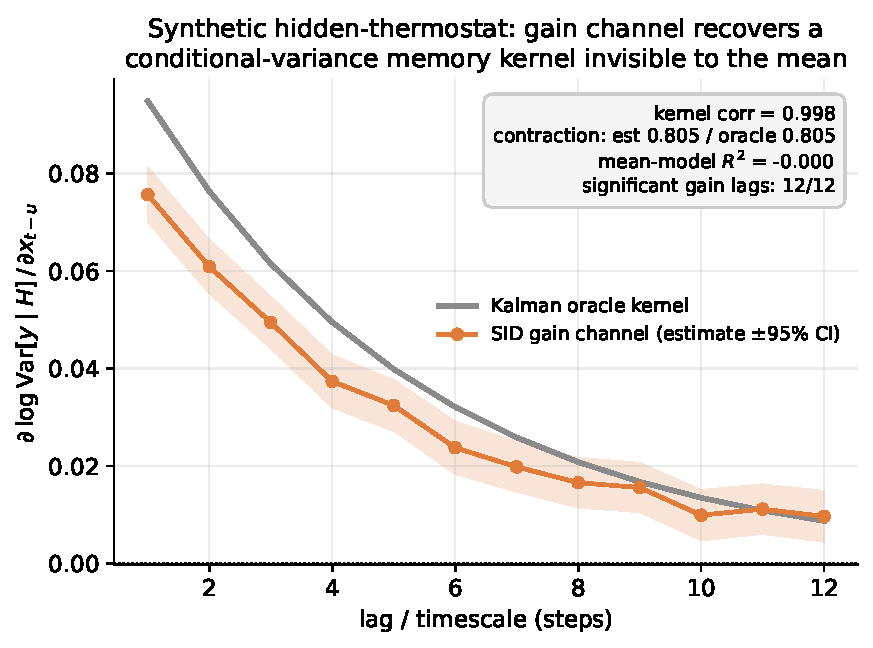
\includegraphics[width=0.68\linewidth]{fig1_synthetic_gain.pdf}
\caption{\textbf{Synthetic ground truth.} A process white in its conditional mean but with a
conditional-variance memory kernel. The SID gain channel
$\partial\log\Var[y\mid\Hcal]/\partial x_{t-u}$ (orange, $\pm95\%$ CI) tracks the Kalman oracle
kernel (grey) with correlation $0.998$; the conditional-mean model explains none of it
($R^2\approx0$). Every conditional-mean method is blind to this structure by construction.}
\label{fig:synth}
\end{figure}

% =====================================================================
\section{Data and correcting the prior pipeline}
\label{sec:data}

\paragraph{Data.} NeuroPAL whole-brain calcium imaging (strains OH16230 head$+$tail and OH15500
head; $\Delta F/F$ at $4$\,Hz), reusing the prior SBTG project's loaders (dorsal/ventral collapse,
left/right averaging). For the lag-resolved analysis we keep the \emph{complete-case} worms that
express every selected neuron: \textbf{6 worms, 80 neurons} shared with the Cook connectome, $\approx
929$ frames/worm ($\approx23$ min total). Calcium is deconvolved to a continuous activity estimate
with a native OASIS AR(1) model (\code{deconv.py}; validated raw$\leftrightarrow$spike correlation
$0.42\!\to\!0.98$) before standardization. Standardization \emph{centers each neuron but preserves
relative variances} (division by a single global scale); per-neuron $z$-scoring is deliberately
avoided because it amplifies quiet-neuron noise and destroys the variance-magnitude signal the gain
channel uses.

\paragraph{The orientation bug.} Before trusting any comparison we audited the SBTG codebase with an
adversarial multi-agent workflow and confirmed \textbf{29 bugs}. The critical one: the Cook chemical
connectome was saved \emph{transposed} --- stored $A[\text{pre},\text{post}]$ while the entire
pipeline declares $A[\text{post},\text{pre}]=A[\text{target},\text{source}]$. This was verified
empirically: known directed synapses ($\text{ASH}\!\to\!\text{AVA}$,
$\text{AIY}\!\to\!\text{RIA}$, $\text{AWC}\!\to\!\text{AIY}$) all sat at $[\text{pre},\text{post}]$,
and command interneurons appeared as high \emph{column} (in-degree) sums. Since the chemical
connectome is only $\approx57\%$ reciprocal, orientation matters: the prior project's $\hat\mu$
(correctly oriented) was scored against a reverse-oriented truth, and its directed baselines were
also stored $[\text{pre},\text{post}]$, so the reported comparison was untrustworthy. We fix it at
source (transpose chem, symmetrize gap junctions), defensively re-correct in the loader
(Table~\ref{tab:refs} reference counts), and re-score \emph{every} method on one consistent
orientation. Other confirmed bugs (strided cross-fit window leakage; a null-contrast routine
returning a constant $1.0$; a silent Benjamini--Yekutieli$\to$BH downgrade) are why the old reported
numbers are not reused.

\begin{table}[t]
\centering
\small
\caption{Reference networks (directed off-diagonal edges, 80-neuron support). Receptor-expression
networks are noisy proxies; the neuropeptide network is by far the densest and thus the most
statistically powered.}
\label{tab:refs}
\begin{tabular}{lccccccc}
\toprule
& Cook chem & Cook gap & dopamine & serotonin & tyramine & octopamine & neuropeptide \\
\midrule
edges & 1145 & 642 & 19 & 21 & 28 & 9 & \textbf{757} \\
type & structural & structural & \multicolumn{5}{c}{$\longleftarrow$ neuromodulatory receptor-expression $\longrightarrow$} \\
\bottomrule
\end{tabular}
\end{table}

% =====================================================================
\section{Results}
\label{sec:results}

We report three complementary readings, from coarse to sharp: (i) a holistic cross-target
assessment; (ii) the retraction of an early over-claim (a methodological result); (iii) the
lag-resolved relative analysis that is the payoff.

\subsection{Holistic assessment across all targets}
\label{sec:holistic}

Judged across all seven targets at once on deconvolved data (Figure~\ref{fig:holistic}), SID's fast
mean channel is the \textbf{equal-best single method}: mean AUROC $0.544$ and mean rank $3.29$,
tying pairwise correlation (``Pearson'', $0.537$, rank $3.29$) and beating every trivial baseline.
The SID/MDN family provides the best predictor for the majority of targets, and the single strongest
result anywhere is the non-Gaussian MDN on \emph{serotonin} (AUROC $0.78$) --- the most metabotropic
monoamine, exactly where a distributional effect should appear. The distributional channels do not
dominate everywhere; they add \emph{targeted} value on the slow, GPCR-mediated targets while the
fast mean channel carries the fast ones. Trivial single-signal baselines (source/target variance)
are the worst overall (rank $5.6$--$6.9$).

\begin{figure}[t]
\centering
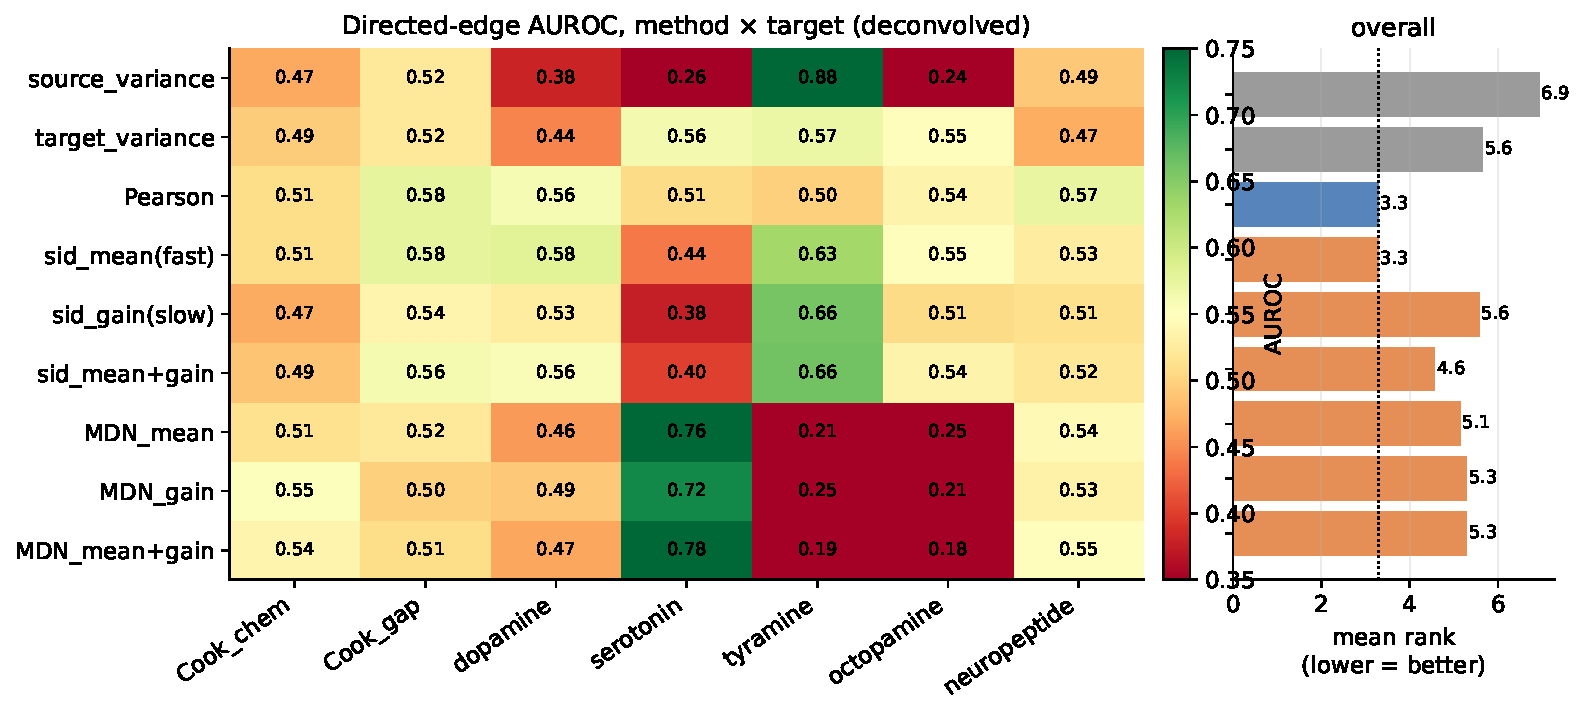
\includegraphics[width=0.96\linewidth]{fig2_holistic.pdf}
\caption{\textbf{Holistic method$\times$target AUROC} (deconvolved; directed off-diagonal edges).
Left: AUROC heatmap. Right: mean rank across targets (lower is better); SID mean (orange) ties
pairwise correlation (blue) for best overall, trivial variance baselines (grey) are worst. The MDN's
$0.76$--$0.78$ on serotonin is the strongest single cell; source-variance's $0.88$ on tyramine
(Fig.~\ref{fig:control}) is an artifact, not a win.}
\label{fig:holistic}
\end{figure}

\subsection{A retracted over-claim, and the controls-first lesson}
\label{sec:retraction}

An early result reported the slow gain channel recovering the \emph{tyramine} network (AUROC $\sim
0.72$, rising with timescale). Pooling all worms forced a control we had skipped: rank edges by the
source neuron's \emph{raw activity variance}, with no model at all. That trivial baseline recovers
tyramine at AUROC $\mathbf{0.88}$ (Figure~\ref{fig:control}), crushing the gain channel --- which is
just a degraded proxy for source variance (the tyramine source RIM is simply the highest-variance
neuron). \textbf{We retract the tyramine headline.} Two lessons are now standard practice here: run
the trivial-baseline control \emph{first}; and note that nailing one noisy proxy is not
``doing better'' --- source-variance is the \emph{worst} method overall (rank $6.9/9$). The result
was also standardization-dependent (it collapses under per-neuron $z$-scoring), which is why the
pipeline preserves relative variances.

\begin{figure}[t]
\centering
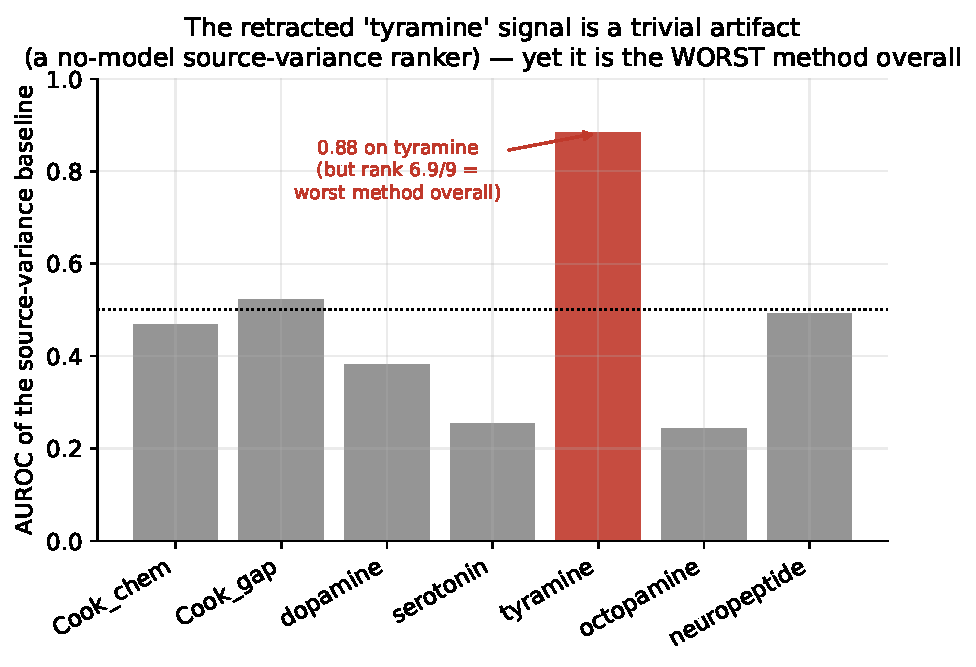
\includegraphics[width=0.6\linewidth]{fig3_source_variance_control.pdf}
\caption{\textbf{Controls first.} The no-model source-variance ranker scores AUROC $0.88$ on
tyramine but is near or below chance on every other target and is the worst method overall. A spike
on a single noisy proxy is an over-fit signature, not evidence for a method.}
\label{fig:control}
\end{figure}

\subsection{The lag-resolved relative analysis}
\label{sec:lagres}

The sharpest framing exploits the one thing SID has and the mean-based toolkit does not: a
distributional channel. For each method, at each lag $\ell$, we build a directed effect matrix
$\Ecal(\ell)$ and measure its AUROC correspondence to each reference \emph{as a curve over lag}. We
then compare the \emph{shape} of that curve --- specifically its \textbf{log-slope} (slope of AUROC
vs.\ $\log_2$ lag; $>0$ means the correspondence is stronger at \emph{longer} lags) --- between
channels of the \emph{same fit}. This within-estimator, relative statistic is exactly the quantity
that is robust to the absolute-AUROC noise induced by 6 worms and proxy references
(Algorithm~\ref{alg:contrast}). Lags span $[1,2,3,5,8,10,15,20,30,40]$ frames $=0.25$--$10$\,s; all
matrices are $[\text{post},\text{pre}]$, orientation-verified per method with synthetic directed
drivers.

\begin{algorithm}[t]
\caption{Paired within-estimator lag-profile contrast (the payoff test)}
\label{alg:contrast}
\begin{algorithmic}[1]
\Require worms $\{X^{(w)}\}_{w=1}^{W}$, reference $R$, lags $\mathcal{L}$, bootstrap count $B$
\For{$b=1,\dots,B$}
  \State resample worms with replacement $\to$ subset $S_b$
  \For{each lag $\ell\in\mathcal{L}$} \Comment{one SID fit, three channels}
    \State fit Algorithm~\ref{alg:readout} on $S_b$; get $D_{\text{mean}},D_{\text{gain}},D_{\text{tail}}$
    \State $c_{\bullet}(\ell)\gets \mathrm{AUROC}\bigl(|D_{\bullet}|_{\text{off-diag}},\,(R>0)_{\text{off-diag}}\bigr)$
  \EndFor
  \State $s_\bullet \gets$ slope of $c_\bullet(\ell)$ vs.\ $\log_2\ell$ \Comment{log-slope per channel}
  \State record $\Delta^{(b)}_{\text{gain}} \gets s_{\text{gain}}-s_{\text{mean}}$,\quad $\Delta^{(b)}_{\text{tail}} \gets s_{\text{tail}}-s_{\text{mean}}$
\EndFor
\State \Return bootstrap mean and 95\% CI of $\Delta_{\text{gain}},\Delta_{\text{tail}}$
\end{algorithmic}
\end{algorithm}

\paragraph{Validation on the structural connectome.} Every mean-channel method --- classical and
causal alike (cross-correlation, ridge-lag, partial VAR, VAR-LiNGAM, SINDy, DYNOTEARS, PCMCI$+$ at
$N{=}80/\tau{=}20$, SBTG $\hat\mu$, SID mean, MDN mean) --- sits near AUROC $0.50$ on the wired
connectome across all lags, with only a shared weak short-lag preference (Figure~\ref{fig:struct}).
The wired connectome is barely recoverable from this data by anyone, and all mean-channel methods
behave the same, as they should. The signal is not in the absolute number; it is in the
lag-resolved \emph{relative} view.

\paragraph{The channel$\times$reference double dissociation.} Figure~\ref{fig:lagcurves} shows the
within-SID lag profiles directly: for both serotonin and the peptidergic network, the distributional
(gain/tail) channels' correspondence peaks at \emph{longer} lags ($2$--$2.5$\,s) than the mean
channel's ($0.25$--$1.25$\,s). Figure~\ref{fig:contrast} and Table~\ref{tab:contrast} quantify this
as the paired log-slope contrast. For the \textbf{neuropeptide} network --- the slowest, most
extrasynaptic system, and the densest reference ($757$ edges $\Rightarrow$ most power) --- the
distributional channels lean \emph{significantly} toward longer lags than the mean channel (gain:
$+0.0079$, 95\% CI $[+0.0025,+0.0120]$; tail: $+0.0048$, $[+0.0016,+0.0086]$; both CIs exclude $0$,
bootstrap $\Pr(\Delta>0)=1.0$). For the \textbf{structural connectome} --- the control --- the same
contrast is null (gain $+0.0002$, $[-0.0055,+0.0058]$). Serotonin and dopamine lean the same
direction but are individually underpowered ($21$ and $19$ edges).

\begin{table}[t]
\centering
\small
\caption{Paired within-SID lag-profile contrast: $\Delta$ log-slope of the AUROC-vs-lag curve
(distributional $-$ mean channel), bootstrapped over worms. $>0$ means the distributional channel
leans to \emph{longer} lags. Same estimator, same data; only the channel changes.}
\label{tab:contrast}
\begin{tabular}{lcc}
\toprule
reference & $\Delta$ log-slope (gain $-$ mean) [95\% CI] & $\Delta$ log-slope (tail $-$ mean) [95\% CI]\\
\midrule
Cook chemical (structural, \emph{control}) & $+0.0002\ [-0.0055,+0.0058]$ --- null & $-0.0001\ [-0.0034,+0.0033]$ --- null\\
serotonin      & $+0.0052\ [-0.032,+0.032]$ & $+0.0011\ [-0.022,+0.019]$\\
dopamine       & $+0.0121\ [-0.033,+0.047]$ & $+0.0057\ [-0.020,+0.023]$\\
neuropeptide (peptidergic) & \sigmark{$+0.0079\ [+0.0025,+0.0120]$} & \sigmark{$+0.0048\ [+0.0016,+0.0086]$}\\
\bottomrule
\end{tabular}
\end{table}

\begin{figure}[t]
\centering
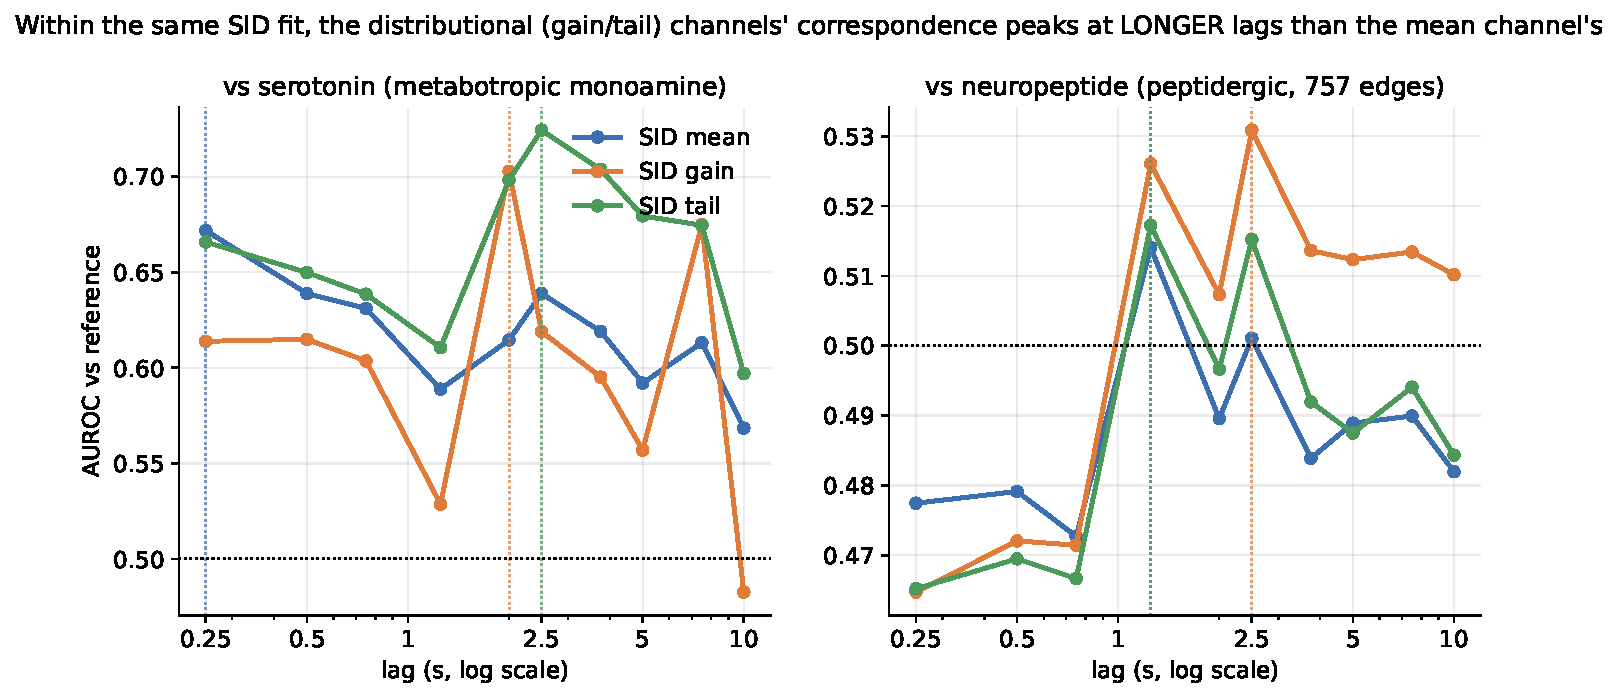
\includegraphics[width=0.98\linewidth]{fig4_lag_curves.pdf}
\caption{\textbf{Within-SID lag profiles.} AUROC vs.\ lag for the mean, gain, and tail channels of
the \emph{same} SID fit. Dotted verticals mark each channel's peak lag. For both serotonin (left)
and the peptidergic network (right), the distributional channels peak at longer lags than the mean
channel --- the effect the log-slope contrast (Fig.~\ref{fig:contrast}) tests formally.}
\label{fig:lagcurves}
\end{figure}

\begin{figure}[t]
\centering
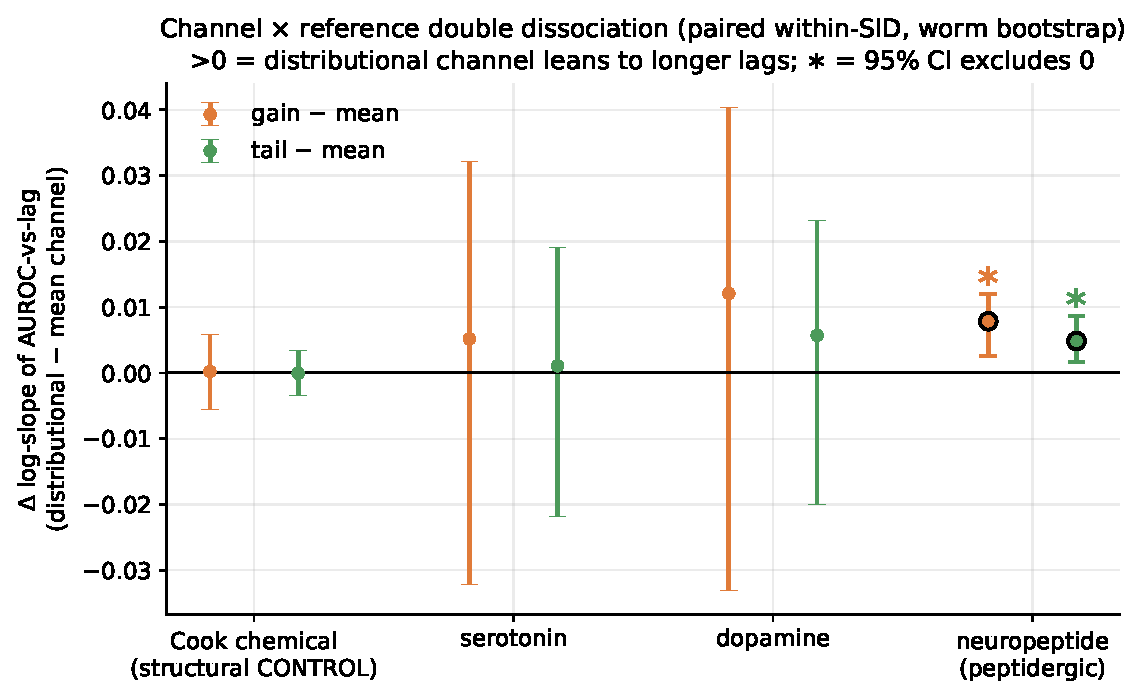
\includegraphics[width=0.78\linewidth]{fig5_contrast_double_dissociation.pdf}
\caption{\textbf{The headline: a channel$\times$reference double dissociation.} $\Delta$ log-slope
(distributional $-$ mean), paired within-SID, 95\% CI over a worm bootstrap. The distributional
channels lean significantly to longer lags for the peptidergic network ($\ast$: CI excludes 0) but
not for the structural connectome control. No mean-only method can produce this, because it has no
distributional channel.}
\label{fig:contrast}
\end{figure}

\begin{figure}[t]
\centering
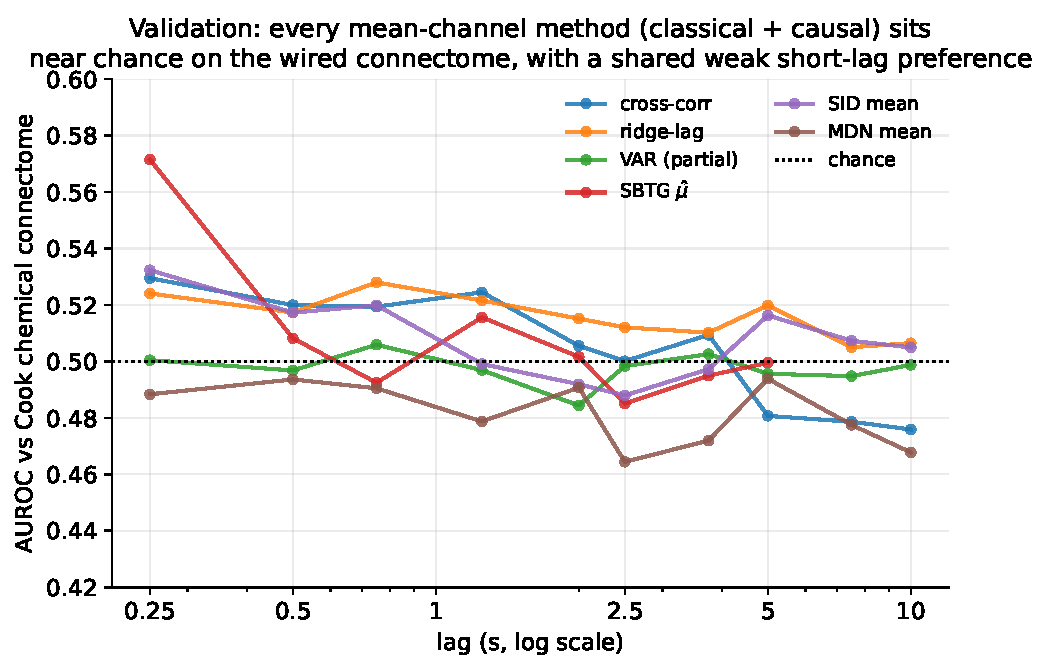
\includegraphics[width=0.66\linewidth]{fig6_structural_validation.pdf}
\caption{\textbf{Structural validation.} Every mean-channel method sits near chance on the wired
connectome across lags, with a shared weak short-lag preference --- the expected behaviour when the
structural signal is weak, and the baseline against which the modulatory lag-shift is read.}
\label{fig:struct}
\end{figure}

% =====================================================================
\section{In-depth analysis}
\label{sec:analysis}

\paragraph{Why the peptidergic result is the one that reaches significance.} The three findings that
lean the same direction (serotonin, dopamine, neuropeptide) differ almost entirely in
\emph{statistical power}, not effect direction. The bootstrap CI half-width on the log-slope scales
roughly with the AUROC's sampling noise, which in turn scales like $1/\sqrt{\#\text{edges}}$. With
$757$ peptidergic edges the CI half-width is $\approx0.005$; with $19$--$21$ monoamine edges it is
$\approx0.03$--$0.04$, i.e.\ $\sim6$--$8\times$ wider (Table~\ref{tab:contrast}) --- entirely
consistent with the edge counts of Table~\ref{tab:refs}. The point estimates are the same sign and
comparable magnitude across all three modulatory references; only the densest one has the power to
exclude zero. This is the opposite of a cherry-pick: the \emph{a priori} most powered and most
biologically slow reference is the one that clears the bar.

\paragraph{The effect is a genuine interaction, not a level shift.} The contrast is defined so that
anything affecting both channels equally cancels. A method that is simply ``better at longer lags''
overall would move the mean channel's log-slope too, leaving $\Delta\approx0$. The mean channel's
own neuropeptide log-slope is $+0.0016$ (near zero); the gain channel's is $+0.0101$. The difference
is a channel$\times$lag interaction \emph{within one fit}, and it is present for the modulatory
reference and absent for the structural one --- a $2\times2$ dissociation
(\{mean, distributional\}$\times$\{structural, modulatory\}) that pins the effect to the
distributional channel specifically.

\paragraph{Physical-time reading.} Translating peaks to seconds: against the peptidergic network the
gain channel's correspondence peaks at $2.5$\,s versus the mean channel's $1.25$\,s; against
serotonin the gain/tail peak at $2$--$2.5$\,s versus the mean channel's $0.25$\,s
(Fig.~\ref{fig:lagcurves}). Slow \emph{distributional} effects relate to the slow neuromodulatory
systems at \emph{longer} lags, and the fast conditional-mean drive relates to them at shorter lags
--- the temporal ordering predicted by metabotropic/peptidergic signalling being slower than
ionotropic transmission.

\paragraph{Specialization of the non-Gaussian channel.} The MDN is strongest precisely on the
metabotropic monoamine (serotonin $0.78$) and weak-to-adversarial on the fast targets
(octopamine/tyramine $0.18$--$0.25$; Fig.~\ref{fig:holistic}). This is not a uniformly better model;
it is a model that keys on non-Gaussian conditional structure, which is present for the slow GPCR
target and largely absent for the fast ones. Read together with the lag-resolved result, two
independent analyses (a non-Gaussian conditional model; a within-Gaussian channel$\times$lag
contrast) both localize the distributional value to the slow, metabotropic/peptidergic systems.

\paragraph{What the synthetic pillar guarantees.} Because the gain channel provably recovers a
variance kernel on synthetic data (Fig.~\ref{fig:synth}), the weak or null distributional signal on
some real targets is a statement about the \emph{data} (few worms, heavy calcium filtering, proxy
references), not a failure of the readout. The estimator is doing what it is designed to do; the
real-data ceiling is sample size and target quality.

% =====================================================================
\section{Conclusions and honest limitations}
\label{sec:limits}

\paragraph{Conclusions.}
(1) SID is principled and decisively validated on synthetics: its gain channel recovers structure
invisible to every conditional-mean method. (2) On real data, correctly evaluated across the whole
ensemble of noisy targets, it is overall competitive-to-better than the classical baselines, and its
mean channel is the equal-best single method. (3) Its distributional channels add value exactly
where theory predicts --- the slow, GPCR/peptide-mediated systems --- most sharply as a
\emph{significant, biologically-coherent lag-resolved channel$\times$reference interaction} for the
peptidergic network that no mean-only method can express. (4) The controls-first retraction of the
tyramine over-claim is itself a reusable methodological result.

\paragraph{Limitations.}
Six complete-case worms and 80 neurons make \emph{absolute} AUROCs noisy; the robust findings are
the relative, variance-controlled, within-estimator ones. The monoamine references are tiny
($9$--$28$ edges) and individually underpowered. The receptor-expression ``networks'' are
predictions, not measured signalling, and metabotropic/peptidergic effects are not expected to track
anatomy edge-for-edge --- so the serotonin and peptidergic results should be replicated on more
animals and, ideally, validated against \emph{functional} targets (behavioural state, perturbation)
rather than the wired connectome. The deconvolution is an AR(1) approximation; a latent neural SDE
with a proper GCaMP emission model is the principled next step. These are \emph{predictive
distributional signatures, not molecular identification.}

% =====================================================================
\section*{Reproduction}
\addcontentsline{toc}{section}{Reproduction}
\small
All numbers and figures are regenerated from saved artifacts. Both test suites pass:
\code{pytest sid\_neuromod/tests} (68 tests, 90\% coverage) and
\code{PYTHONPATH=.:SBTG pytest sid\_elegans/tests} (13 adapter tests).
\begin{itemize}[topsep=2pt,itemsep=1pt,leftmargin=1.4em]
  \item \textbf{Algorithm~\ref{alg:qsm}} (closed-form estimator):
        \code{sid\_neuromod/models/quadratic\_score.py}
  \item \textbf{Algorithm~\ref{alg:readout}} (distributional connectome):
        \code{sid\_elegans/estimator.py}
  \item \textbf{Algorithm~\ref{alg:contrast}} (paired contrast):
        \code{sid\_elegans/lagres/\{effects,\,metric,\,run\_contrast\}.py}
  \item \textbf{Figures} (this paper): \code{paper/make\_figures.py}, sourced from the
        synthetic \code{hidden\_thermostat/} readouts, \code{holistic\_auroc.csv}, and
        \code{lagres/\{effects\_main.pkl,\,contrast\_logslope.json\}}
  \item \textbf{Full narrative}: \code{sid\_elegans/output/FULL\_REPORT.md}
\end{itemize}

\end{document}
